\documentclass{beamer}
\usepackage{beamerthemeshadow}
\usepackage{graphicx}
\usepackage{color}
\usepackage[utf8]{inputenc}
\usepackage[english, serbian]{babel} 
\usepackage{hyperref}
\usepackage[flushleft]{threeparttable}
\definecolor{beamer@darkred}{rgb}{0.75,0.5,0.1}
\setbeamercolor{structure}{fg=beamer@darkred}

\def\d{{\fontencoding{T1}\selectfont\dj}}
\def\D{{\fontencoding{T1}\selectfont\DJ}}


\title{Tehničko i naučno pisanje}
\subtitle{-- Tehnološka Singularnost --}
\author{Nikola Ahac, Dimitrije Petronijević, Mladen Radojević, Lazar Stošić}
\institute{Matematički fakultet\\Univerzitet u Beogradu}
\date{
	\footnotesize{Beograd, 2022.}	
}

\begin{document}
\begin{frame}
	\thispagestyle{empty}
	\titlepage
\end{frame}

\addtocounter{framenumber}{-1}

\begin{frame}[fragile]\frametitle{Literatura}
	\begin{itemize}
		\item Zasnovano na:\\
		The Technological Singularity, Murray Shanahan.
	\end{itemize}
\end{frame}

\begin{frame}
	\frametitle{Pregled} % Table of contents slide, comment this block out to remove it
	\tableofcontents[hidesubsections] 
\end{frame}
\section{Uvod}

\begin{frame}[fragile]\frametitle{Uvod}
	\begin{itemize}	
		\item Pojam "Tehnološka singularnost".
		\item Vernor Vindž (eng. Vernor Vinge)
              
              \textit {"Kada čovek stvori mašinu koja je pametnija od čoveka, budućnost će postati nepredvidiva, jer je nemoguće predvideti ponašanje inteligencije koja je superijornija od čovekove."}

	\end{itemize}
\end{frame}

\section{Istorija}
\begin{frame}[fragile]\frametitle{Istorija}
    \begin{itemize}	
        \item Prva osoba koja je upotrebila koncept „singularnosti“ u tehnološkom kontekstu bio je Džon fon Nojman(eng.\textit{John von Neumann}).
        \item Koncept i termin singularnost popularizovao je Vernor Vinge 1993. godine.
	 \item Neki naučnici, uključujući Stivena Hokinga(eng. \textit{Stephen Hawking}), izrazili su zabrinutost da bi veštačka superinteligencija mogla dovesti do izumiranja ljudi.
    \end{itemize}
\end{frame}


\section{Kako i kada će doći do singularnosti}
\subsection{Pojava super inteligencije}
\begin{frame}[fragile]\frametitle{Pojava super inteligencije}
	\begin{itemize}	
		\item Pojam ''Super inteligencije" ili "Nadljudske inteligencije".
        \item Moguća scenarija i posledice .
        \item Knjiga "The Age of Em" Robina Hansona.
	\end{itemize}
\end{frame}

\subsection{Singularnost bez veštačke inteligencije}
\begin{frame}[fragile]\frametitle{Singularnost bez veštačke inteligencije}
	\begin{itemize}	
        \item Postoji grupa naučnika i pisaca koja smatra da do singularnosti može doći i bez "veštačke super inteligencije"
        \item Vindž i naučnici koji se slažu sa njim navode da bez tehnološke ''super inteligencije" takve promene ne bi mogle da se kvalifikuju kao singularnost.
	\end{itemize}
\end{frame}

\subsection{Brza superinteligencija}
\begin{frame}[fragile]\frametitle{Brza superinteligencija}
	\begin{itemize}	
        \item "Brza superinteligencija", je veštačka inteligencija koja funkcioniše isto kao i naš um, samo dosta brže.
        \item Ako bi se tehnološkim napretkom došlo do ovoga, to bi mogao biti okidač singularnosti.
	\end{itemize}
\end{frame}
\section{Verovatnoća}

\begin{frame}[fragile]\frametitle{Verovatnoća da će doći do singularnosti}
    \begin{itemize}	
        \item Glavni faktori:
        \begin{itemize}	
            \item Poboljšivači inteligencije
            \item Otežavanje tehnološkog napretka
            \item Eventualna fizička granica
      \end{itemize}
    \end{itemize}
\end{frame}

\begin{frame}[fragile]\frametitle{Razvoj brzine tehnološkog napretka}
    \begin{itemize}	
        \item Murov zakon (eng. Moore's Law)
        \item Kurcvailov zakon o ubrzanom povratku
    \end{itemize}
    \begin{figure}[h!]
        \centering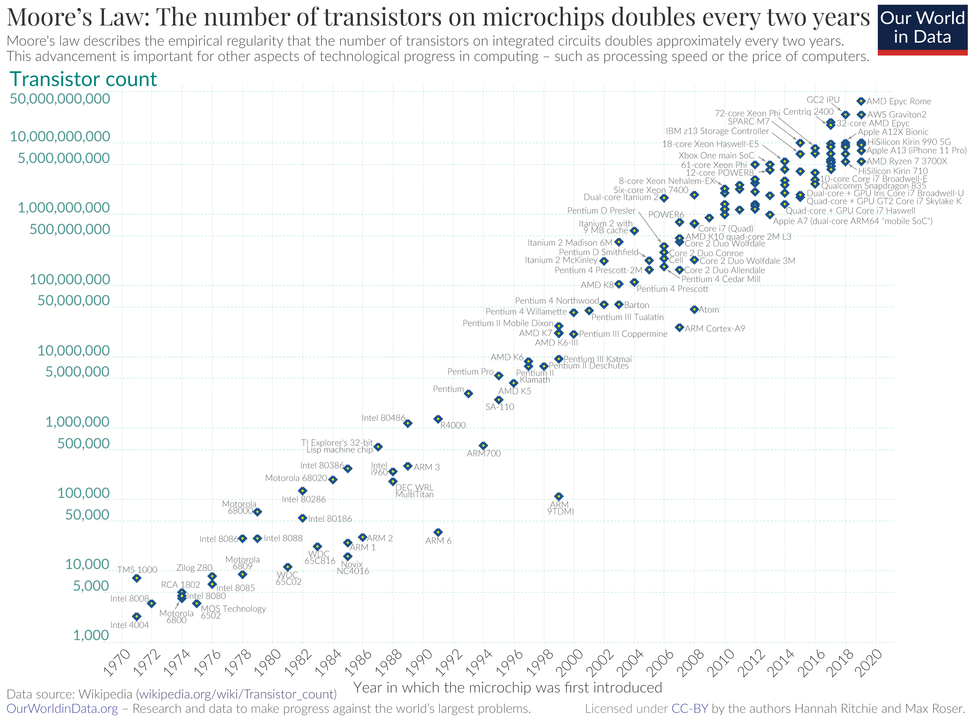
\includegraphics[height=5cm]{moore.png} 
        \caption{Grafik Murovog zakon}
        \label{fig:murovzakon}
    \end{figure}
\end{frame}


\begin{frame}[fragile]\frametitle{Razvoj algoritama}
    \begin{itemize}	
        \item Kako se razlikuje od čistog povećanja brzine izvršavanja?
        \item Seed AI
    \end{itemize}
\end{frame}

\section{Potencijalni uticaj ekonomskog rasta}
\begin{frame}[fragile]\frametitle{Potencijalni uticaj ekonomskog rasta}
	\begin{itemize}	
		\item Brzina rasta ekonomije kroz vreme
            \begin{itemize}
                \item Paleolit-Neolit: ekonomija se duplirala na svakih 250.000 godina.
                \item Poljoprivredna ekonomija: duplirala se na svakih 900 godina.
                \item Industrijska revolucija-savremeno doba: ekonomija se duplirala na svakih 15 godina.
            \end{itemize}   
            \item Superinteligencija bi izazvala dupliranje na nedeljnoj bazi.
	\end{itemize}
\end{frame}

\subsection{Nestabilnost i rizik}
\begin{frame}[fragile]\frametitle{Nestabilnost i rizik}
	\begin{itemize}	
            \item "Uspeh u stvaranju veštačke inteligencije bi bio najveći uspeh u ljudskoj istoriji. Nažalost, to bi veorovatno bio i poslednji, osim ako ne naučimo kako da izbegnemo rizike."

	\end{itemize}
\end{frame}

\subsection{Trenutno stanje evolucije}
\begin{frame}[fragile]\frametitle{Trenutno stanje evolucije}
	\begin{itemize}	
		\item Tehnološska singularnost je viđena kao događaj koji se dešsava tek tako od
jednom
            \item Neki naučcnici tvrde da je trenutna brzina evolucije perfektna takva kakva
jeste.
	\end{itemize}
 
        \begin{table}[h!]
            \begin{center}
                \begin{tabular}{|c|c|} \hline
                    \textbf{godina}& \textbf{količina podataka (zetabajt)}\\ \hline
                        1980 &0.0026 ZB\\ \hline
                        1993 &0.0158 ZB\\ \hline
                        2000 &0.0545 ZB\\ \hline
                        2007 &0.2950 ZB\\ \hline
                        2014 &5.0000 ZB\\ \hline
                        2020 &6.8000 ZB\\ \hline
                \end{tabular}
            \caption{Eksponencijalni rast broja digitalnih informacija kroz godine.}
            \label{tab:tabela1}
            \end{center}
        \end{table}
\end{frame}
\subsection{Besmrtnost}
\begin{frame}[fragile]\frametitle{Besmtnost}
	\begin{itemize}	
        \item Tehnološki napredak u medicini
        \item Povećanje ljudskog životnog veka
        \item Ričardu Fejman i Albert Hibs – korišćenje Feynman-ovih teoretskih mikromašina u okviru medicine.
        \item "Digital Ascension" (eng. digitalno uzdizanje)
	\end{itemize}
\end{frame}
\section{Teško i lako poletanje}

\begin{frame}[fragile]\frametitle{Teško i lako poletanje}
	\begin{itemize}	
		\item Kada i ako dode do tehnološke singularnosti, postoje dva moguća scenarija:
  \begin{itemize}
  \item Teško poletanje 
  \item  Lako poletanje
  \end{itemize}
		\item Ramez Naam na temu teškog poletanja
		\item Česti scenariji teškog poletanja - Džon Stors Hol
	\end{itemize}
\end{frame}

\section{Tema "Tehnološka singularnost" u politici}

\begin{frame}[fragile]\frametitle{Tema "Tehnološka singularnost" u politici}
	\begin{itemize}	
		\item Zajednički ekonomski komitet Kongresa Sjedinjenih Američkih Država na temu tehnološke singularnosti  i nanotehnologije
		\item Bivši predsetnik Sjedinjenih Američkih Država Barak Obama(eng.\textit{Barack Obama} ) na intervjuu časopisa Wired 2016. godine na temu tehnološke singularnosti.
		\item Nekritička pretpostavka vlade SAD-a da će se odjednom "sve promeniti" u bliskoj budućnosti.
	\end{itemize}
\end{frame}

\section{Zakljucak}

\begin{frame}[fragile]\frametitle{Zaključak}
\begin{itemize}	
 \item Otkiće veštačke inteligencije je unapredilo savremeno društvo  u raznim aspektima, možemo videti razna poboljšanja u granama medicine, građevine i mnogih drugih zanimanja, ali veštačka inteligencija nastavlja da se razvija i ne planira da se zaustavi. Mi možemo samo da spekulišemo kada će doći do singularnosti.
\item Da li će ljudi naizad dostići neograničen životni vek? Da li će veštačka inteligencija prevazići čoveka u svakom aspektu rada? Da li će kompjuteri preuzeti svet u budućnosti?

\end{itemize}
\end{frame}

\end{document}
